\pdfoutput=1
\pdfcompresslevel=9
\pdfinfo
{
    /Title (Rozproszony system plików)
    /Subject (Rozproszone systemy operacyjne)
    /Keywords (dfs rozproszony hdfs gfs system plików)
}
%\documentclass[a4paper,polish,onecolumn,oneside,floatssmall,11pt,titleauthor,wide,openright]{mwrep}
%\usepackage[scale={0.7,0.8},paper=a4paper,twoside]{geometry}
\documentclass[a4paper,onecolumn,oneside,11pt,wide,floatssmall]{mwrep}
% \usepackage{polish}
\usepackage{amsmath}
\usepackage{amsfonts}
\usepackage{amssymb}
\usepackage{amsthm}
\usepackage{bookman}
%dodane przez nme
\usepackage{float}
\usepackage{pifont}% http://ctan.org/pkg/pifont

\usepackage{geometry}
\usepackage[utf8x]{inputenc}
\usepackage[T1]{fontenc}
% \usepackage{t1enc}
% \usepackage[pdftex, bookmarks]{hyperref}
\usepackage[pdftex, bookmarks=false]{hyperref}
\def\url#1{{ \tt #1}}

\usepackage{listings}

% marginesy
\textwidth\paperwidth
\advance\textwidth -55mm
\oddsidemargin-0.9in
\advance\oddsidemargin 33mm
\evensidemargin-0.9in
\advance\evensidemargin 33mm
\topmargin -1in
\advance\topmargin 25mm
\setlength\textheight{48\baselineskip}
\addtolength\textheight{\topskip}
\marginparwidth15mm

\clubpenalty=10000 % to kara za sierotki
\widowpenalty=10000 % nie pozostawia wdów
\brokenpenalty=10000 % nie dzieli wyrazów pomiędzy stronami
\sloppy

\tolerance4500
\pretolerance250
\hfuzz=1.5pt
\hbadness1450

% ŻYWA PAGINA
\renewcommand{\chaptermark}[1]{\markboth{\scshape\small\bfseries \
#1}{\small\bfseries \ #1}}
\renewcommand{\sectionmark}[1]{\markboth{\scshape\small\bfseries\thesection.\
#1}{\small\bfseries\thesection.\ #1}}
\newcommand{\headrulewidth}{0.5pt}
\newcommand{\footrulewidth}{0.pt}
\pagestyle{uheadings}

\renewcommand{\labelitemi}{$\bullet$}

\usepackage[pdftex]{color,graphicx}
\usepackage[polish]{babel}
\usepackage[none]{hyphenat}%%%%
\usepackage{setspace}
% \textheight232mm
% \setlength{\textwidth}{\textwidth}
% \setlength{\oddsidemargin}{\evensidemargin}
% \setlength{\evensidemargin}{0.3cm}
\usepackage[sort, compress]{cite}

%\usepackage{multibib}
%\newcites{bk,st,doc,web}{Książki i~artykuły,Standardy i~zalecenia,Dokumentacja produktów,Publikacje i~serwisy internetowe}

\theoremstyle{definition}
\newtheorem{defn}{Definicja}[section]
\newtheorem{conj}{Teza}[section]
\newtheorem{conjmain}{Teza}
\newtheorem{exmp}{Przykład}[section]

\theoremstyle{plain}% default
\newtheorem{thm}{Twierdzenie}[section]
\newtheorem{lem}[thm]{Lemat}
\newtheorem{prop}[thm]{Hipoteza}
\newtheorem*{cor}{Wniosek}

\theoremstyle{remark}
\newtheorem*{rem}{Uwaga}
\newtheorem*{note}{Uwaga}
\newtheorem{case}{Przypadek}

\definecolor{ListingBackground}{rgb}{0.95,0.95,0.95}

\begin{document}

% kody źródłowe wplatane w tekst
\lstdefinestyle{incode}
{
basicstyle={\small},
keywordstyle={\bf\color{black}},
commentstyle={\em\color{black}},
numbers=left,
stepnumber=1,
firstnumber=1,
numberfirstline=true,
numberblanklines=true,
numberstyle={\sf\tiny},
numbersep=10pt,
tabsize=2,
xleftmargin=17pt,
framexleftmargin=3pt,
framexbottommargin=2pt,
framextopmargin=5pt,
framexrightmargin=0pt,
showstringspaces=true,
backgroundcolor={\color{ListingBackground}},
extendedchars=true,
% title=\lstname,
captionpos=b,
% abovecaptionskip=1pt,
% belowcaptionskip=1pt,
frame=tb,
framerule=0pt
}

% kody źródłowe z podpisem
\lstdefinestyle{outcode}
{
basicstyle={\footnotesize},
keywordstyle={\bf\footnotesize\color{blue}},
commentstyle={\em\footnotesize\color{magenta}},
numbers=left,
stepnumber=5,
firstnumber=1,
numberfirstline=true,
numberblanklines=true,
numberstyle={\sf\tiny},
numbersep=10pt,
tabsize=2,
xleftmargin=17pt,
framexleftmargin=3pt,
framexbottommargin=2pt,
framextopmargin=2pt,
framexrightmargin=0pt,
showstringspaces=true,
backgroundcolor={\color{ListingBackground}},
extendedchars=true,
% title=\lstname,
captionpos=b,
% abovecaptionskip=1pt,
% belowcaptionskip=1pt,
frame=tb,
framerule=0.1pt,
}

\renewcommand*\lstlistingname{Wydruk}
\renewcommand*\lstlistlistingname{Spis wydruków}
\renewcommand*\tablename{Tabela}

\pagenumbering{roman}
\renewcommand{\baselinestretch}{1.0}
\raggedbottom

\setstretch{1.2}

\begin{titlepage}
    % Strona tytułowa
    \vbox to\textheight{\hyphenpenalty=10000
    \begin{center}
	\vspace*{3.75\baselineskip}
	\par\vspace{\smallskipamount}
	\vspace*{2\baselineskip}{\huge\bfseries Rozporszone Systemy Operacyjne\par}
	\vspace{3\baselineskip}{\LARGE\strut Rozproszony system plików - Etap III\par}

	\vspace*{7\baselineskip}
	\hfill\mbox{}\par\vspace*{\baselineskip}\noindent
	\begin{tabular}[b]{@{}p{3cm}@{\ }l@{}}
	    {\large\hfill } & {\large }
	\end{tabular}
	\hfill
	\begin{tabular}[b]{@{}l@{}}
		\textbf{Skład zespołu:} \\[\smallskipamount]
	Marcin Dzieżyc \\
	Piotr Kalinowski \\
	Adam Papros \\
	Mateusz Statkiewicz \\
	Marcin Swend \\
	Jacek Witkowski
	\end{tabular}\par
    \end{center}}

\end{titlepage}


\tableofcontents
% \addcontentsline{toc}{chapter}{{Przedmowa1}{vii}}{vii}

% \chapter*{Spis tablic, rysunków i~wydruków}
% \listoftables
% \listoffigures
% \lstlistoflistings

%\setlength{\baselineskip}{7mm}
\newpage
\pagenumbering{arabic}
\setcounter{page}{1}

\chapter[Opis rozwiązania Apache Thrift][Opis rozwiązania Apache Thrift]{Opis
rozwiązania Apache Thrift}

Thrift to narzędzie, którego głównym celem jest umożliwienie tworzenia
skalowanych oraz interoperacyjnych usług. Biblioteka ta~pierwotnie została
na~otwartej licencji Apache 2.0
zaimplementowana i~była używana przez Facebooka, ale~aktualnie jest dostępna
(http://www.apache.org/licenses/LICENSE-2.0.html).

\vspace{5mm}
Thrift dzięki prostemu językowi IDL (język opisu interfejsu ang.~\emph{Interface
Definition Language}) pozwala definiować oraz tworzyć usługi dla~wielu
popularnych i~rozwijanych języków programowania. W~oparciu o~plik w~języku IDL
niezależny od~języka programowania Thrift generuje biblioteki służące
do~transportu danych pomiędzy klientem a~serwerem, wystawiając do~nich
odpowiednie interfejsy. Programista zajmuje się~jedynie implementacją
faktycznego działania aplikacji w~oderwaniu od~sposobów przekazywania danych,
co~sprawia, że~tworzenie rozwiązań w~oparciu o~RPC (zdalne wywołanie procedury,
ang.~\emph{Remote Procedure Call}) jest bardzo proste.

\section[Architektura Apache Thrift][Architektura Apache Thrift]{Architektura
Apache Thrift}
\begin{figure}[H]
\center
\flushleft
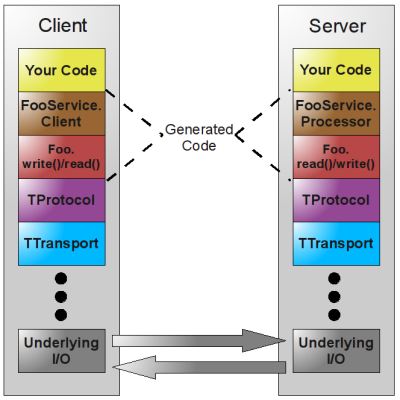
\includegraphics[keepaspectratio=true]{img/thrift_arch.png}
\caption{Źródło: http://jnb.ociweb.com/jnb/jnbJun2009.html}
\label{fig:thriftArch}
\end{figure}

\vspace{5mm}
Diagram przedstawia stos warstw implementacyjnych, które umożliwiają
komunikację RPC zgodnie z filozofią Apache Thrift.  Pierwsze trzy górne warstwy
stanowią kod napisany w tym samym języku, dla którego kompilator IDL Apache
Thrift wygenerował kod. Pierwsza warstwa to kod użytkownika-programisty, który
wykorzystuje dostarczoną abstrakcję RPC. Dwie następne warstwy to wygenerowany
kod realizujący pożądane przez użytkownika usługi. Pozostałe, niższe warstwy są
niezależne od pliku opisu interfejsu - wykorzystywany jest kod bibliotek
odpowiednich do realizacji komunikacji.

\section[Apache Thrift IDL][Apache Thrift IDL]{Apache Thrift IDL}
\hspace*{-\parindent}%
\begin{minipage}{\linewidth}
\subsection[Wspierane podstawowe typy danych][Wspierane podstawowe typy
danych]{Wspierane podstawowe typy danych}
\begin{itemize}
	\item \textbf{bool} - wartość logiczna 
	\item \textbf{byte} - bajt ze znakiem
	\item \textbf{i16} - 16 bitowa liczba całkowita ze znakiem
	\item \textbf{i32} - 32 bitowa liczba całkowita ze znakiem
	\item \textbf{i64} - 64 bitowa liczba całkowita ze znakiem
	\item \textbf{double} - 64 bitowa liczba zmienno pozycyjna
	\item \textbf{string} - tekstowy typ danych
\end{itemize}
\end{minipage}

\subsection[Kontenery][Kontenery]{Kontenery}
\hspace*{-\parindent}%
\begin{minipage}{\linewidth}
Thrift umożliwia definiowanie zbiorów danych przy pomocy trzech rodzajów
kontenerów:
\begin{itemize}
	\item \textbf{list}<typ> - uporządkowana kolekcja 
	\item \textbf{set}<typ> - nieuporządkowana kolekcja
	\item \textbf{map}<typ\_klucza, typ\_wartości>  - mapa
	klucz-wartość
\end{itemize}
\end{minipage}

\subsection[Struktury][Struktury]{Struktury}
Thrift umożliwa definiowanie złożonych struktur danych przypominających
struktury z języka C. Definiuje się je w następujący sposób:
\begin{lstlisting}[language=C, style=incode]
struct <nazwa_struktury>
{
	1:<typ_danych_1> <nazwa_skladowej_1>,
	2:<typ_danych_2> <nazwa_skladowej_2>,
	3:<typ_danych_3> <nazwa_skladowej_3>,
}
\end{lstlisting}

\subsection[Wyjątki][Wyjątki]{Wyjątki}
Deklarowanie wyjątków jest podobne do~definiowania struktur.

\begin{lstlisting}[language=C, style=incode, morekeywords={exception}]
exception <nazwa_wyjatku>
{
	1:<typ_danych_1> <nazwa_skladowej_1>,
	2:<typ_danych_2> <nazwa_skladowej_2>,
	3:<typ_danych_3> <nazwa_skladowej_3>,
}
\end{lstlisting}

\newpage
\section[Zalety korzystania z rozwiązania Apache Thrift][Zalety korzystania z
rozwiązania Apache Thrift]{Zalety korzystania z rozwiązania Apache Thrift}
Wykorzystanie Apache Thrift posiada wiele zalet z~perspektywy programisty:
\begin{itemize}
  \item posiada czytelny dla~człowieka, niezależny od~języka plik opisu
  interfejsu,
  \item umożliwia zmianę protokołu i~sposobu transportu danych bez~poważnych
  zmian w~kodzie - wykorzystywane są~możliwości narzędzia Apache Thrift,
  \item zapewnia wysoką wydajność serializacji pomiędzy różnymi językami
  (w~porównaniu do~popularnych protokołów wykorzystujących XML lub~JSON) przez
  możliwość wykorzystania protokołu binarnego,
  \item serwer wielowątkowy (lub~jednowątkowy), wykorzystujący funkcje blokujące
  lub~nieblokujące dostępny ,,prosto z pudełka''.
\end{itemize}

\chapter[Uruchomienie dostępnych w sieci przykładów demonstrujących
wykorzystanie Apache Thrift][Uruchomienie dostępnych w sieci przykładów
demonstrujących wykorzystanie Apache Thrift]{Uruchomienie dostępnych w sieci
przykładów demonstrujących wykorzystanie Apache Thrift}
Jednym z~etapów dobrego poznania Apache Thrift, było uruchomienie dostępnych
w~sieci przykładów wykorzystujących to~narzędzie. Kolejnym krokiem, była
implementacja prostej usługi przypominającej bardzo uproszczone zadanie
projektowe. Uruchomionym przykładem demonstrującym wykorzystanie Apache Thrift
był ,,Thrift by Example'' ze strony:
\emph{http://thrift-tutorial.readthedocs.org/en/latest/usage-example.html}.

\vspace{5mm}
Opisano sposób realizacji prostej usługi zapewniającej operacje matematyczne.
Przykład wprowadza do:
\begin{itemize}
  \item składni oraz możliwości języka opisu interfejsu dla narzędzia - Thrift
  IDL,
  \item sposobu użycia kompilatora Thrift IDL,
  \item sposobu implementacji aplikacji klienta w języku Java,
  \item sposobu implementacji aplikacji serwera wraz z odpowiednimi klasami
  realizującymi usługę w języku Java,
  \item przykład dodatkowo opisuje sposób nawiązywania bezpiecznych połaczeń
  (przy pomocy SSL).
\end{itemize}

\vspace{5mm}
Przykładowa usługa umożliwia klientowi zapytanie serwera o wynik operacji -
w~ramach zdalnego wywołania procedury klient przekazywał argumenty oraz typ
operacji. Dodatkowo wykorzystano mechanizmy Apache Thrift umożliwiające
rzucanie wyjątków (na~przykład w przypadku próby dzielenia przez 0).

\vspace{5mm}
Demonstracja Thrift by Example wprowadza w Apache Thrift, pokazuje przykładowe
zastosowanie i~proponuje przykładową implementację wykorzystującą to~narzędzie.

\vspace{5mm}
Drugim elementem wprowadzenia do Apache Thrifta była samodzielna implementacja
bardzo uproszczonej wersji usługi, o której mowa w zadaniu projektowym
-~rozproszonego systemu plików. W~ramach tych prac powstały dwie grupy usług:
NamingService oraz StorageService, które odpowiadają kolejno warstwie usług
lokalizacyjno-nazewniczej oraz warstwie właściwego przechowywania.

\hspace*{-\parindent}%
\begin{minipage}{\linewidth}
\begin{lstlisting}[
language=C,
style=incode,
caption={Interfejs serwera nazewniczego},
morekeywords={typedef,int,service,string,namespace}]
namespace java NamingService
typedef i32 int

service NamingService
{
	int put(1:string fileName),
	int get(1:string fileName)
}
\end{lstlisting}
\end{minipage}

\hspace*{-\parindent}%
\begin{minipage}{\linewidth}
\begin{lstlisting}[
language=C,
style=incode,
caption={Interfejs serwera przechowującego dane},
morekeywords={typedef,int,service,string,namespace,byte}]
namespace java StorageService
typedef i32 int

service StorageService
{
        void putFile(1:int fileId, 2:list<byte> body),
        list<byte> getFile(1:int fileId)
}
\end{lstlisting}
\end{minipage}

\vspace{5mm}
Aplikacja kliencka, gdy~chce wysłać plik do~systemu plików, najpierw łączy
się~z~serwerem nazewniczym -~w~tym~momencie zostaje zrealizowane zarejestrowanie
nazwy oraz przypisanie identyfikatora pliku. W~drugim kroku aplikacja kliencka
łączy się~z~serwerem przechowującym dane, przesyła identyfikator pliku (nadany
przez serwer nazewniczy) oraz kolekcje bajtów (ciało pliku).
\chapter[Przegląd istniejących rozwiązań][Przegląd istniejących
rozwiązań]{Przegląd istniejących rozwiązań}
Obecnie na rynku istnieje wiele dostępnych rozproszonych systemów plików,
zarówno komercyjnych, jak~i~darmowych. Swoje implementacje takich systemów
oferuje większość znaczących firm informatycznych, takich jak~Microsoft,
Google, Apache, Oracle, IBM czy RedHat. Poniżej zaprezentowane zostały dwa
wybrane rozproszone systemy plików.

\section[Google File System (GFS)][Google File System (GFS)]{Google File System
(GFS)}
GFS został zaprojektowany na~wewnętrzne potrzeby firmy Google, aby~przechowywać
duże ilości danych związanych z~pracą wyszukiwarki internetowej. W~systemie
wyróżnić można dwa rodzaje serwerów: Master oraz Chunkserver. Zadaniem tych
drugich jest przechowywanie wszystkich plików w~systemie. Pliki są~gromadzone
w~blokach (ang.~\emph{chunk}), każdy o~wielkości 64 megabajtów, które
replikowane są~pomiędzy kilkoma Chunkserverami (minimum trzy). Podczas operacji
czytania lub~przesyłania plików klient komunikuje się~bezpośrednio z~tymi serwerami.

\vspace{5mm}
Serwer Master jest z~kolei odpowiedzialny za~trzymanie wszystkich metadanych
o~plikach, czyli takich informacji jak odwzorowanie 64-bitowych etykiet plików
na~ich~lokalizację na~Chunk Serverach, lokalizację kopii bloków danych oraz
informacje o aktualnych operacjach wejścia i wyjścia w systemie. Wszystkie
te~dane są~aktualizowane poprzez periodycznie wysyłane komunikaty od~każdego z~serwerów.

\vspace{5mm}
Poniżej znajduje się schemat rozwiązania GFS:

\begin{figure}[H]
\center
\flushleft
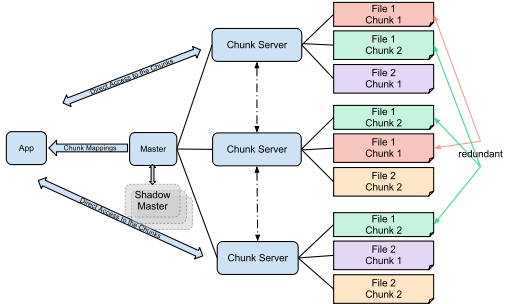
\includegraphics[keepaspectratio=true, scale=0.9]{img/gfs.png}
\caption{Źródło: http://en.wikipedia.org/wiki/Google\_File\_System}
\label{fig:gfs}
\end{figure}

\section[Hadoop File System (HDFS)][Hadoop File System (HDFS)]{Hadoop File
System (HDFS)}
Głównymi cechami, które wyróżniają ten rozproszony system plików od~innych jest
wysoka odporność na~błędy oraz skuteczność działania na~mniej wydajnym
sprzęcie. System ten~wchodzi w~skład rozwiązania open-source zwanego Apache Hadoop.

\vspace{5mm}
Podobnie jak~GFS, Hadoop File System składa się~z~głównego serwera zwanego
Namenode, który odpowiada za~usługi nazewnicze i~lokalizacyjne plików oraz
udostępnia interfejs dla~klienta. Dane są~przechowywane na~serwerach zwanych
Datanodes. Są~również pomiędzy nimi replikowane. Pliki mogą być przechowywane
w~całości lub~we~fragmentach.

\vspace{5mm}
Poniżej przedstawiony został schemat architektury HDFS:

\begin{figure}[H]
\center
\flushleft
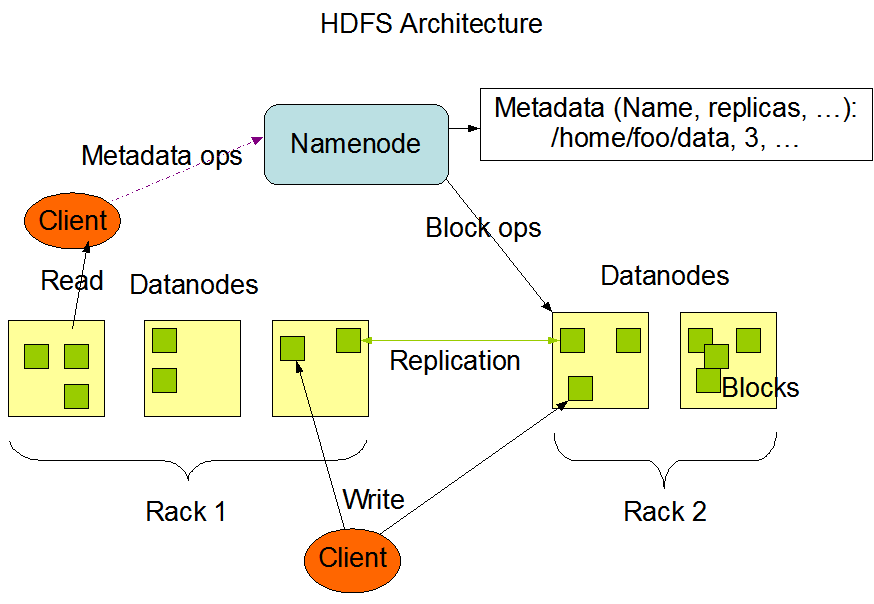
\includegraphics[keepaspectratio=true, scale=0.45]{img/hdfs.png}
\caption{Źródło: http://hadoop.apache.org/docs/r1.2.1/hdfs\_design.html}
\label{fig:hdfs}
\end{figure}

Lista innych przykładowych rozproszonych systemów plików:
\begin{itemize}
  \item Ceph (Inktank),
  \item FhGFS (Fraunhofer),
  \item GlusterFS (RedHat),
  \item Lustre,
  \item Windows Distributed File System (Microsoft).
\end{itemize}

\vspace{5mm}
Na przykładzie GFS oraz HDFS można zauwazyć, że~ogólny zamysł architektoniczny
rozproszonych systemów plików jest dość podobny. Większym różnicom podlegają
szczególy implementacyjne.
\chapter[Koncepcja rozwiązania własnego][Koncepcja rozwiązania
własnego]{Koncepcja rozwiązania własnego}
Zadaniem projektowym jest wytworzenie rozproszonego systemu plików
przechowującego pliki w~pamięci operacyjnej bądź na~dyskach lokalnych. System
implementowany przez nasz zespół będzie przechowywał pliki na~dyskach lokalnych.

\vspace{5mm}
Usługa podzielona jest na~2 warstwy:
\begin{itemize}
  \item warstwa usług lokalizacyjno-nazewniczych (Master Server),
  \item warstwa właściwego przechowywania (Storage Server).
\end{itemize}

\vspace{5mm}
System opiera się~na~następującej architekturze:
\begin{figure}[H]
\center
\flushleft
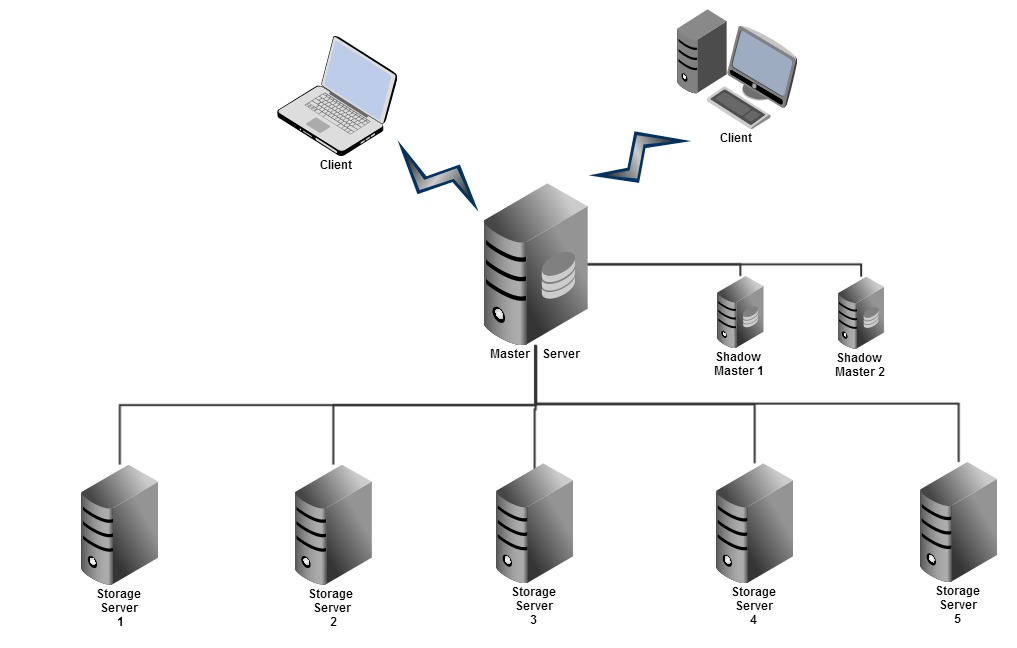
\includegraphics[keepaspectratio=true, scale=0.45]{img/own_conception.png}
\end{figure}

\vspace{5mm}
Master Server odpowiada za~kontakt z~klientem oraz za~przydzielanie plików
do~odpowiednich Storage Serverów. Dodatkowo zarządza bazami danych na~serwerach
lustrzanych (Shadow Server).

\vspace{5mm}
W bazach przechowywane jest drzewo plików załadowanych do systemu, wraz
z~ich~fizycznym miejscem położenia -~identyfikatorami Storage Serverów.

\vspace{5mm}
System zapewnia niezawodność poprzez replikację plików, oraz kopie Master
Servera. Skalowalność jest zapewniona przez~łatwe dołączanie kolejnych Storage
Serverów bez~strat w~wydajności systemu. Rozważano koncepcję odciążenia Master
Servera w~przypadku operacji nie~zmieniających stanu plików (get, status),
które mogły by~być~wykonywane przez~Shadow Servery, jednak dla~zachowania
prostoty zdecydowano by~nie realizować tej~koncepcji.

\vspace{5mm}
System pozwala klientowi ładować pliki do~systemu, pobierać je, usuwać oraz
sprawdzać ich~stan. Podstawowe operacje przedstawiono na~poniższych diagramach:

\begin{figure}[H]
\center
\flushleft
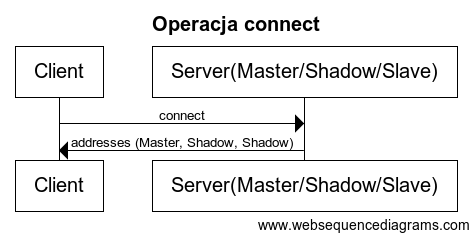
\includegraphics[keepaspectratio=true, scale=0.5]{img/connect_op.png}
\end{figure}

\begin{figure}[H]
\center
\flushleft
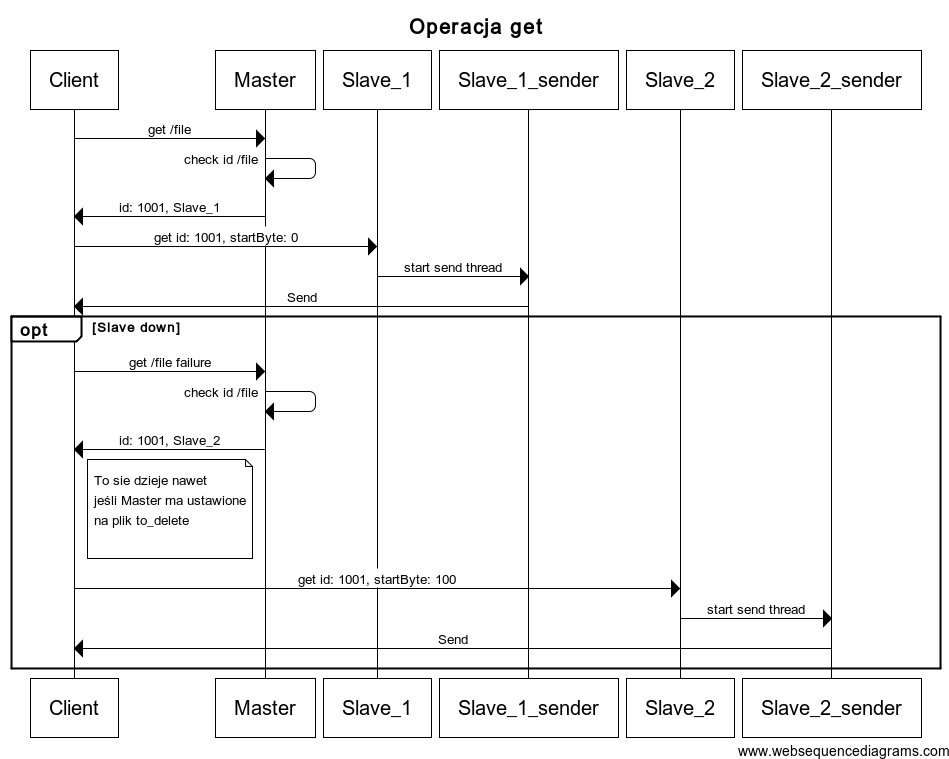
\includegraphics[keepaspectratio=true, scale=0.47]{img/get_op.png}
\end{figure}

\begin{figure}[H]
\center
\flushleft
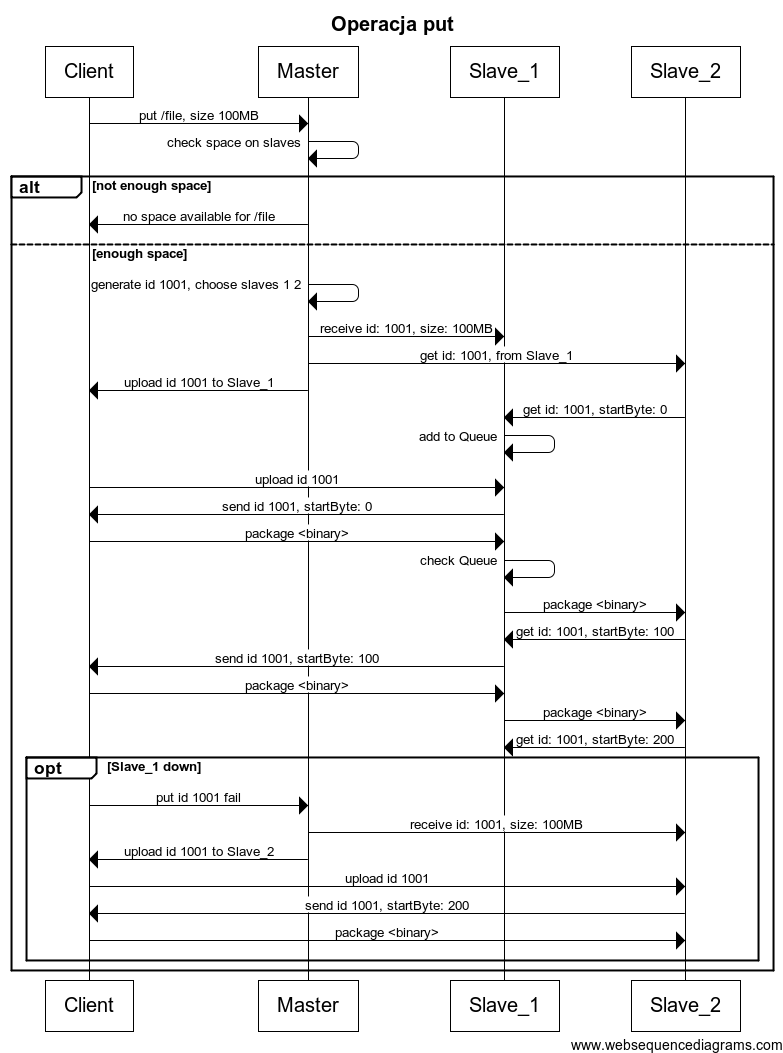
\includegraphics[keepaspectratio=true, scale=0.5]{img/put_op.png}
\end{figure}

\begin{figure}[H]
\center
\flushleft
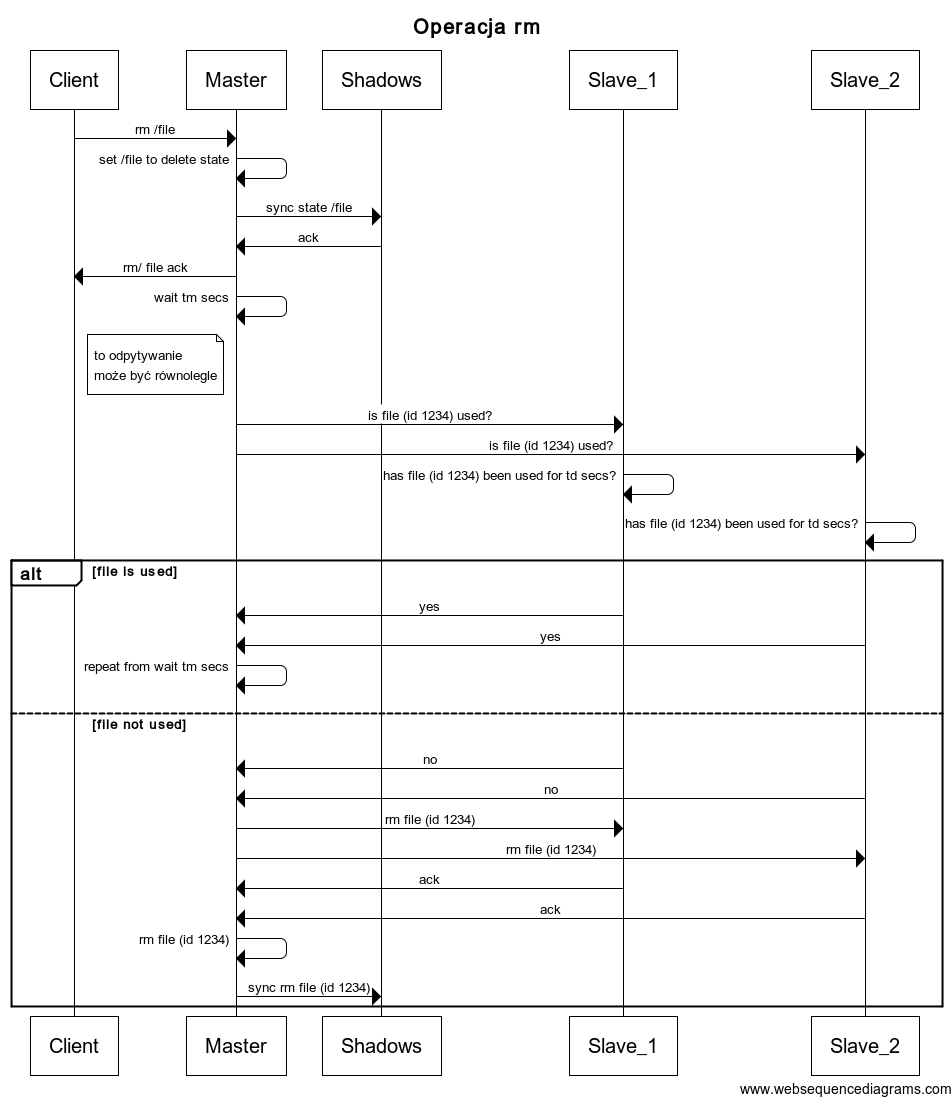
\includegraphics[keepaspectratio=true, scale=0.47]{img/rm_op.png}
\end{figure}

Od strony administratorskiej -~początkowe serwery są~włączane za~pomocą skryptu
uruchamiającego usługę. Operacja przyłączenia nowego serwera, który przez
określony czas nie~odpowiadał, przebiega w~następujący sposób:
\begin{figure}[H]
\center
\flushleft
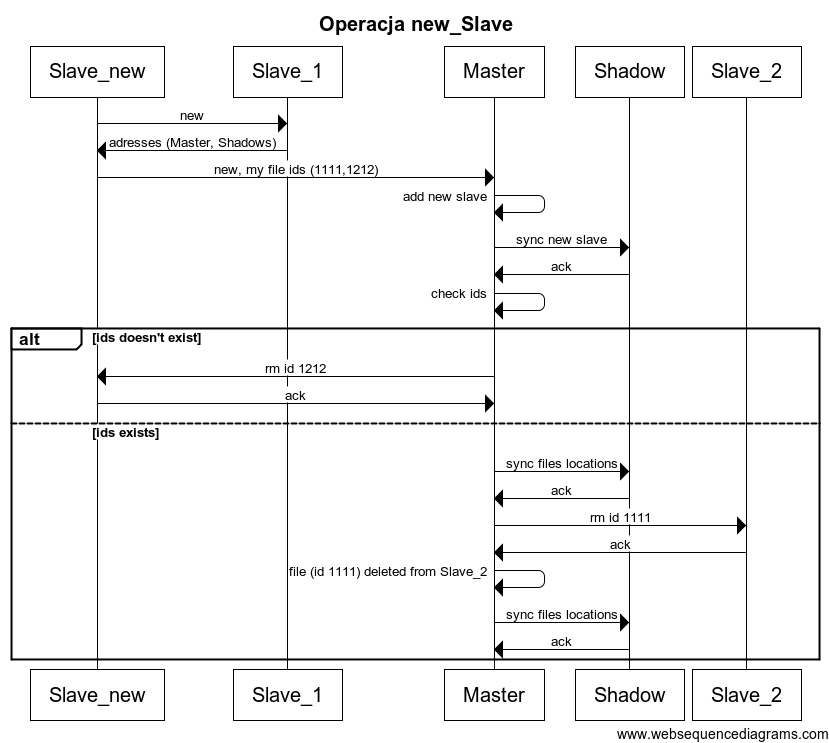
\includegraphics[keepaspectratio=true, scale=0.5]{img/new_slave_op.png}
\end{figure}
\chapter[Implementacja][Implementacja]{Implementacja}
Podczas prac nad systemem powstały takie artefakty jak:
\begin{itemize}
  \item skrypt uruchamiający usługę,
  \item aplikacja kliencka,
  \item aplikacja serwerowa,
  \item skrypt demostracyjny.
\end{itemize}

\section[Interfejs usługi][Interfejs usługi]{Interfejs usługi}
W~ramach prac nad~systemem opracowano API zdefiniowane w~języku Apache
Thrift~IDL, które przedstawiono na~poniższym wydruku:

\begin{lstlisting}[language=C,style=incode,
morekeywords={exception,typedef,i32,i64,namespace,enum,required,struct,bool}]
namespace java rso.dfs.generated

typedef i32 int
typedef i64 long
typedef string IPType

enum ServerType {
	Slave,
	Master,
	Shadow
}

struct ServerStatus
{
	1: required ServerType type;
	2: required i32 filesNumber;
	3: required i64 freeSpace;
	4: required i64 usedSpace;
	5: required IPType serverIP;
}

struct SystemStatus {
	1:required i32 filesNumber;
	2:required list<ServerStatus> serversStatuses;
}

struct CoreStatus {
	1:IPType masterAddress;
	2:list<IPType> shadowsAddresses;
}

// describes part of file
struct FilePartDescription {
	1:int fileId;
	2:long offset;
}

//represents part of a file
struct FilePart {
	1:int fileId;
	2:long offset;
	3:binary data;
}

// communication initiated by new node
// new node sends to master file list
struct NewSlaveRequest {
	1:required IPType slaveIP;
	2:list<int> fileIds;
	3:list<long> fileSizes;
}
struct GetFileParams
{
	1:required i32 fileId;
	2:required IPType slaveIp;
	3:required i64 size;
}

struct PutFileParams
{
	1:required bool canPut;
	2:required i32 fileId;
	3:required IPType slaveIp;
}

service Service
{
	//returns administrative system status
	SystemStatus getStatus(),
	
	// returns list of file names 
	list<string> listFileNames(),
	
	//infrastucure building
	//slave sends request to master to register to serve
	CoreStatus registerSlave(1:NewSlaveRequest req),
	
	//with this request master makes slave register again.
	void forceRegister(1:CoreStatus status),
	
	//master updates slaves status
	void updateCoreStatus(1:CoreStatus status),
	
	//master sends request to slave
	void becomeShadow(1: CoreStatus status),
	
	//client - anyone
	CoreStatus getCoreStatus(), // returns master/shadows list
	
	//ping server for checking whether it's alive
	void pingServer(),
	
	// file id, file size; master slave
	// force slave to be ready for file (fileId)
	// which will be sent from client
	void prepareForReceiving(1: int fileID, 2:long size),
	//file id, slave ip
	void replicate(1:int fileID, 2:IPType slaveIP, 3:long size),
	
	//master - slave
	bool isFileUsed(1:int fileID),
	void removeFileSlave(1:int fileID),
	
	GetFileParams getFile(1:string filepath),
	GetFileParams getFileFailure(1:string filepath),
	PutFileParams putFile(1:string filepath, 2:long size),
	PutFileParams putFileFailure(1:string filepath, 2:long size),
	bool removeFile(1:string filepath),
	
	// returns: which part of file should be sent next
	FilePartDescription sendFileToSlaveRequest(1: int fileId),
	
	// Input: part of file which has to be sent
	// returns: which part of file should be sent next,
	//          special value in case of finish
	FilePartDescription sendFilePartToSlave(1: FilePart filePart),
	FilePart getFileFromSlave(1: FilePartDescription filePartDescription),
	
	void fileUploadSuccess(1:int fileID, 2: IPType slaveIP) 
}
\end{lstlisting}

\section[Zarządzanie usługą][Zarządzanie usługą]{Zarządzanie usługą}
Podczas prac nad~systemem wytworzono skrypt powłoki (\emph{shell script})
ułatwiający zarządzanie usługą. Umożliwa on~m.in.~uruchamianie oraz
zatrzymywanie usługi, a~także pozwala wyświetlić informacje o~bieżącym stanie
usługi. W~celu korzystania ze~skryptu konieczne jest posiadanie systemu
z~rodziny Unix z~zainstalowanymi narzędziami: \emph{awk, timeout oraz nmap}.
Możliwe wywołania skryptu zamieszczono na~poniższym zestawieniu.

\vspace{5mm}
\renewcommand{\arraystretch}{1.5}
\begin{tabular}[h]{p{3cm} p{11cm}}
\emph{start}	[timeout] & próbuje uruchomić \emph{naming service} na~każdym z~IP,
po~pierwszym sukcesie uruchamia slave'y. Implementacja daje [timeout
w~milisekundach] milisekund (domyślnie 5000) na~uruchomienie się~aplikacji serwera od~chwili wykonania komendy ssh. \\
\emph{stop} & zatrzymuje usługę \\
haltvm & zatrzymuje każdy z~serwerów (wykonuje na~nim polecenie powłoki
\emph{halt}) \\
\emph{status} & uruchamia \emph{system status} dla~pierwszego~servera, z~którym
uda się~zkomunikować \\
\emph{client} & nawiązuje połączenie z~pierwszym serwerem, z~którym uda
się~zkomunikować \\
\end{tabular}
\chapter[Scenariusze testowe][Scenariusze testowe]{Scenariusze testowe}
Testowanie oprogramowania będzie polegało na~wywoływaniu szeregu scenariuszy
powiązanych z~możliwymi usterkami występującymi podczas działania systemu
zarówno z~powodu wystąpienia sytuacji nadzwyczajnych, jak~i~z~powodów
zewnętrznych, nie~związanych z błędami w~samym oprogramowaniu. Scenariusze będą
polegały na~wywoływaniu operacji po~stronie klienta, a~następnie symulacji
objawów usterek związanych z~zadanym scenariuszem testowym; weryfikacja testu
odbywać się~będzie na~podstawie porównania reakcji systemu z~oczekiwanymi
poprawnymi reakcjami na~wysłanie żądania. Potencjalne błędy, które testy będą
musiały sprawdzić, obejmują w~szczególności problemy synchronizacyjne:
opóźnienia oraz desynchronizację, ale~również najczęściej spotykane usterki
nie~powiązane z~zagadnieniami rozproszonymi.

\begin{table}[h]
\begin{center}
	\begin{tabular}{|p{4cm} | p{4cm} | p{6cm} |}
		\hline
		\textbf{Scenariusz} & \textbf{Możliwe powody} &	\textbf{Rozwiązanie}	\\	\hline
		Timeout             & Podany serwer jest niedostępny &	Ponowne przeszukanie
		puli dostępnych serwerów \\ \hline
		Odpowiedź: IP serwerów typu Master i Shadow & Klient podłączył się~do~innego
		serwera niż~master & Nawiązanie połączenia z~masterem na~podstawie otrzymanych
		danych \\ \hline
		Klient otrzymuje niewłaściwe adresy - próbuje połączyć się~do~serwera
		o~niepoprawnym~typie & Opóźnienie propagacji, zmiana serwera master.
		& Ponowne odpytanie serwerów ze~znanej puli shadow. \\ \hline
	\end{tabular}
\end{center}
\caption{Scenariusze dla operacji \emph{connect (Client -> Server)}}
\end{table}

\begin{table}[h]
\begin{center}
	\begin{tabular}{|p{4cm} | p{4cm} | p{6cm} |}
		\hline
		\textbf{Scenariusz} & \textbf{Możliwe powody} &	\textbf{Rozwiązanie}	\\	\hline
		File not found      & Master nie może znaleźć pliku w~bazie lub plik ma
		ustawiony tryb do~usunięcia &	(Klient) Sprawdzić poprawność ścieżki oraz
		sprawdzić listing plików \\ \hline
		Slave down (timeout) & Podany serwer jest niedostępny & Wykonanie zwrotnego
		zapytania do mastera w celu wybrania nowego slave’a \\ \hline
		Not enough space (u klienta) & Brak miejsca u~klienta & Zwrócenie błędu \\
		\hline
		
	\end{tabular}
\end{center}
\caption{Scenariusze dla operacji \emph{get}}
\end{table}

\begin{table}[h]
\begin{center}
	\begin{tabular}{|p{4cm} | p{4cm} | p{6cm} |}
		\hline
		\textbf{Scenariusz} & \textbf{Możliwe powody} &	\textbf{Rozwiązanie}	\\	\hline
		Not enough space & Zapełniona przestrzeń dyskowa slave’ów & Usunąć pliki
		z~systemu \\ \hline
		(M-S) Timeout & Wybrany serwer jest niedostępny & Master wybiera nowego
		slave’a do~puli replikacyjnej i~deaktywuje niedostępnego \\ \hline
		(C-S) Timeout & Wybrany slave jest niedostępny & Klient ponawia próbę wysłania
		pliku za~pośrednictwem mastera. Dodatkowo: master wybiera dodatkowy slave
		do~replikacji i~informuje całą resztę o~zmianie lokalizacji repliki głównej.
		\\ \hline
		(S-S) Timeout & Połączenie replikacyjne nie~może zostać ustabilizowane. &
		Master zostaje poinformowany o~zaburzeniu procesu replikacyjnego i~wybiera
		nowe brakujące slave’y do~replikacji. \\ \hline
	\end{tabular}
\end{center}
\caption{Scenariusze dla operacji \emph{put}}
\end{table}

\makeatletter
\setlength{\@fptop}{0pt}
\makeatother
\begin{table}[h]
	\begin{tabular}{|p{4cm} | p{4cm} | p{6cm} |}
		\hline
		\textbf{Scenariusz} & \textbf{Możliwe powody} &	\textbf{Rozwiązanie}	\\	\hline
		File not found. & Plik nie istnieje w systemie. & Zwrócenie błędu \\ \hline
		(M-SM) Timeout & Serwer poboczny jest niedostępny. & Master wywołuje proces
		elekcji serwera pobocznego. \\ \hline
		(M-S) Timeout & Serwer magazynujący jest niedostępny. & Master zamyka
		połączenie; plik zostanie usunięty z~serwera magazynującego podczas kolejnego
		połączenia. \\ \hline
		Master ulega awarii w~trakcie oczekiwania na~slave’y & & Serwer poboczny
		wykonuje zapytanie o pliki do usunięcia z bazy i wznawia proces. \\ \hline
	\end{tabular}
\caption{Scenariusze dla operacji \emph{rm}}
\end{table}
\chapter[Harmonogram realizacji projektu. Przydział ról w projekcie][Harmonogram
realizacji projektu. Przydział ról w projekcie]{Harmonogram realizacji projektu.
Przydział ról w projekcie}
Podczas pierwszego spotkania projektowego ustalono podział ról oraz terminy
przyszłych spotkań. Podział obowiązków ulegał modyfikacjom. Ostatecznie
ustalono następujący przydział ról:
\begin{itemize}
  \item kierownik projektu: Jacek Witkowski,
  \item architekt: Marcin Swend,
  \item zarządca repozytorium: Jacek Witkowski,
  \item dokumentalista: Jacek Witkowski,
  \item tester: Marcin Dzieżyc,
  \item handlowiec: Mateusz Statkiewicz.
\end{itemize}

Oprócz powyżej przydzielonych ról specjalnych, każdy z członków zespołu pełnił
również rolę programisty (za wyjątkiem kierownika projektu). Po analizie wymagań
zawartych w~instrukcji do~projektu dostępnej pod~adresem:
\emph{http://www.ia.pw.edu.pl/~tkruk/edu/rsob2014/lab/rso\_projekt2014.txt}
ustalono następujący harmonogram prac:
\begin{itemize}
  \item \textbf{4~marca 2014}: ustalenie podziału ról oraz organizacji
  środowiska programistycznego projektu,
  \item \textbf{11~marca 2014}: ustalenie funkcjonalności oferowanych przez
  system, ustalenie zawartości pliku konfiguracyjnego, ustalenie zarysu architektury systemu,
  \item \textbf{14~marca 2014}: ustalenie scenariuszy wysyłania i pobierania
  pliku,
  \item \textbf{18~marca 2014}: ustalenie scenariuszy uruchomienia i zamnięcia
  systemu,
  \item \textbf{25~marca 2014}: ustalenie funkcjonalności realizowanych w fazie
  drugiej,
  \item \textbf{1~kwietnia 2014}: przygotowanie wstępnej wersji dokumentacji,
  \item \textbf{4~kwietnia 2014}: opracowanie interfejsów komunikacyjnych
  udostępnianych przez serwer nazewniczy (master), serwer przechowujący (slave) oraz klienta;
  opracowanie komunikatów wymienianych między masterem i slave’em, masterem i
  klientem oraz slave’em i klientem,
  \item \textbf{6~kwietnia 2014}: przygotowanie dokumentacji spełniającej
  wszystkie wymogi dotyczące I etapu projektu,
  \item \textbf{22~kwietnia 2014}: implementacja operacji wysyłania i pobierania
  danych z systemu przy założeniu bezawaryjności urządzeń oraz komunikacji między
  nimi; nie będzie zaimplementowana replikacja; ustalenie pełnego planu testów;
  opracowanie końcowej demonstracji projektu,
  \item \textbf{29~kwietnia 2014}: implementacja operacji usuwania danych,
  \item \textbf{4~maja 2014}: opracowanie wersji dokumentacji spełniającej
  wszystkie wymogi dotyczące II etapu projektu,
  \item \textbf{16~maja 2014}: zapewnienie odpowiedniej niezawodności
  przechowywania danych (m.in. implementacja replikacji plików, uwzględnienie możliwych do
  wystąpienia sytuacji awaryjnych),
  \item \textbf{27~maja 2014}: usunięcie wykrytych błędów istniejących w
  systemie,
  \item \textbf{2~czerwca 2014}: przygotowanie pełnej dokumentacji projektu
  spełniającej wymogi dotyczące III etapu projektu.
\end{itemize}
\chapter[Organizacja środowiska programistycznego projektu][Organizacja
środowiska programistycznego projektu]{Organizacja środowiska programistycznego
projektu}
Podczas wykonywania projektu zostały wykorzystane następujące narzędzia:
\begin{itemize}
  \item \textbf{Git} - jako system kontroli wersji,
  \item \textbf{GitHub} - jako zdalne repozytorium dla narzędzia git,
  \item \textbf{Google Docs} - do~wspólnego tworzenia wstępnej dokumentacji
  projektowej,
  \item \textbf{Latex} - do~przygotowania dokumentacji projektowej,
  \item \textbf{Redmine} - do zarządzania projektem.
\end{itemize}

\vspace{5mm}
Wybór gita jako systemu kontroli wersji był podyktowany prostotą jego
użytkowania oraz wysoką funkcjonalnością. Dodatkowo, wszyscy członkowie zespołu
znają to~narzędzie.

\vspace{5mm}
Kolejny wybór dotyczył zdalnego repozytorium, na~którym miały by~być
przechowywane zasoby z~gita. Wybór padł na~serwis GitHub, gdyż oferuje
on~darmowe usługi dla~projektów niekomercyjnych oraz udostępnia wiele danych
statystycznych pomocnych przy zarządzaniu projektem (np.~wykres aktywności).

\vspace{5mm}
Jako narzędzie do~zarządzania projektem wybrano system Redmine. Jego głównymi
zaletami są:
\begin{itemize}
  \item wysoka funkcjonalność,
  \item możliwość integracji z~innymi systemami (np.~z~systemem kontroli wersji
  git),
  \item łatwość użytkowania.
\end{itemize}
\chapter[Raporty ze spotkań][Raporty ze spotkań]{Raporty ze spotkań}
\section[Spotkanie nr 1][Spotkanie nr 1]{Spotkanie nr 1}

\noindent
\textbf{data}: 2014-03-04 \\
\textbf{czas}: 18:00-18:30

\vspace{5mm}
\noindent
\textbf{uczestnicy}:
\begin{itemize}
	\item Jacek Witkowski
	\item Mateusz Statkiewicz
	\item Marcin Swend
	\item Piotr Kalinowski
\end{itemize}

\vspace{5mm}
\noindent
\textbf{cele}:
\begin{itemize}
  \item Organizacja:
  \begin{itemize}
    \item wymiana danych kontaktowych,
    \item określenie swoich preferencji co~do~ról istniejących w~projekcie,
    \item ustalenie możliwych terminów i formy spotkań.
  \end{itemize}
  \item Wstępna analiza wymagań dotyczących realizacji projektu.
  \item Przegląd i~ewentualny wybór narzędzi używanych podczas realizacji
  projektu.
\end{itemize}

\vspace{5mm}
\noindent
\textbf{ustalenia}: \\
Każdy z członków zespołu określił role projektowe, które chciałby wykonywać.
Wstępnie przyjęto następujący podział ról:
\begin{itemize}
  \item architekt: Marcin Swend,
  \item zarządca repozytorium: Jacek Witkowski,
  \item dokumentalista: Jacek Witkowski,
  \item tester: Mateusz Statkiewicz,
  \item handlowiec: Jacek Witkowski.
\end{itemize}

\vspace{5mm}
Ponadto, każdy z członków zespołu (poza kierownikiem projektu) przyjmuje rolę
programisty.

\vspace{5mm}
Ustalono, że możliwe terminy spotkań to wtorki o godzinie 18.00 oraz piątki
o godzinie 18.00. Istnieje również możliwość odbywania telekonferencji
w weekendy.

\vspace{5mm}
Dokumentacja będzie prowadzona przy użyciu Google Docs, ponieważ każdy
z członków projektu już teraz posiada konto w serwisie Google. Stąd, korzystanie
z narzędzia nie niesie ze sobą konieczności dodatkowego rejestrowania się.
Do~zarządzania projektem zostanie użyty system Redmine, który zostanie
uruchomiony na serwerze Michała Statkiewicza. Jako narzędzie kontroli wersji
zostanie wykorzystany git. Repozytorium zostanie utworzone w serwisie GitHub.

\section[Spotkanie nr 2][Spotkanie nr 2]{Spotkanie nr 2}

\noindent
\textbf{data}: 2014-03-11 \\
\textbf{czas}: 18:00-18:30

\vspace{5mm}
\noindent
\textbf{uczestnicy}:
\begin{itemize}
	\item Jacek Witkowski
	\item Mateusz Statkiewicz
	\item Marcin Swend
	\item Adam Papros
	\item Marcin Dzieżyc
\end{itemize}

\vspace{5mm}
\noindent
\textbf{cele}:
\begin{itemize}
  \item ustalenie wymagań funkcjonalnych projektu,
  \item ustalenie założeń dotyczących środowiska uruchomieniowego,
  \item ustalenie zawartości pliku konfiguracyjnego,
  \item ustalenie wstępnej architektury systemu.
\end{itemize}

\vspace{5mm}
\noindent
\textbf{ustalenia}: \\
Założenia dotyczące projektu:
\begin{itemize}
	\item aplikacja kliencka będzie programem konsolowym,
	\item będą możliwe do użycia następujące komendy:
	\begin{itemize}
		\item ls - wylistowanie zawartości folderu,
		\item cd - zmiana bieżącego katalogu,
		\item rm - usunięcie wskazanego pliku lub folderu,
		\item cp - kopiowanie pliku/folderu z~miejsca źródłowego do~docelowego,
		\item mv - przemieszczenie pliku/folderu z miejsca źródłowego do~docelowego.
   \end{itemize}
\end{itemize}

\vspace{5mm}
Środowisko uruchomieniowe: 4 laptopy działające w~jednej podsieci. 
Laptopy będą połączone za~pomocą routera oferującego możliwość
bezprzewodowego połączenia. Na~laptopach uruchomione będą maszyny wirtualne,
na~których uruchomione będą aplikacje klienckie lub serwerowe.

\vspace{5mm}
\noindent
Spis rzeczy, które muszą znaleźć się w pliku konfiguracyjnym:
\begin{itemize}
  \item lista reprezentująca adresy ip dozwolone dla urządzeń stanowiących
  część serwerową w systemie,
  \item stopień redundancji danych.
\end{itemize}

\vspace{5mm}
\noindent
Wstępna architektura systemu:
\begin{itemize}
  \item urządzenia stanowiące część usługową będą podzielone na dwie klasy:
część lokalizacyjno-nazewniczą oraz cześć przechowawczą,
  \item wśród urządzeń klasy lokalizacyjno-nazewniczej wyróżnione będzie jedno
  urządzenie typu master, które będzie przechowywać informacje o~rozmieszczeniu
  plików w~katalogach oraz o~ich~lokalizacji na~poszczególnych urządzeniach
  przechowawczych.
  \item urządzenia z~klasy lokalizacyjno-nazewniczej nie~będące masterem, będą
  tzw.~\emph{shadow masterami} stanowiącymi dokładną kopię mastera i~będącymi 
  w~stanie go~zastąpić w~razie jego awarii.
\end{itemize}

\section[Spotkanie nr 3][Spotkanie nr 3]{Spotkanie nr 3}

\noindent
\textbf{data}: 2014-03-14 \\
\textbf{czas}: 16:00-18:30

\vspace{5mm}
\noindent
\textbf{uczestnicy}:
\begin{itemize}
	\item Marcin Dzieżyc
	\item Piotr Kalinowski
	\item Adam Papros
	\item Mateusz Statkiewicz
	\item Marcin Swend
	\item Jacek Witkowski
\end{itemize}

\vspace{5mm}
\noindent
\textbf{cele}: \\
Ustalenie scenariuszy dla następujących działań:
\begin{itemize}
  \item wysyłanie pliku,
  \item pobieranie pliku.
\end{itemize}

\vspace{5mm}
\noindent
\textbf{ustalenia}: \\
Scenariusz pobierania pliku:
\begin{enumerate}
	\item Klient łączy się do dowolnego serwera.
	\item Klient otrzymuje adres mastera.
	\item Klient łączy się z masterem.
	\item Klient wydaje polecenie pobrania pliku o określonej ścieżce.
	\item Master wyszukuje plik w hierarchii plików.
	\item Master odsyła do klienta listę slave'ów przechowujących pliki wraz
	z~identyfikatorem pliku.
	\item Klient nawiązuje połączenie z~pierwszym z~listy slave'ów i~wysyła żądanie
	pobrania pliku o~wskazanym identyfikatorze od~zerowego bajta.
	\item Slave rozpoczyna wysyłanie pliku.
	\item Klient odbiera plik.
\end{enumerate}

\vspace{5mm}
Scenariusz wysyłania pliku:
\begin{enumerate}
	\item Klient łączy się do dowolnego serwera.
	\item Klient otrzymuje adres mastera.
	\item Klient łączy się z masterem.
	\item Klient informuje mastera o~chęci wysłania pliku o~określonej ścieżce
	i~rozmiarze.
	\item Master sprawdza czy plik już~istnieje oraz wysyła do~wybranych slave'ów
	informację o~identyfikatorze pliku, który ma~zostać odebrany wraz z~listą
	wszystkich slave'ów, do~których została wysłana ta~lista (każdy z~wybranej
	grupy slave'ów otrzymuje tę~samą listę).
	\item Master wysyła identyfikator pliku i~listę która była rozsyłana w~p.~5
	do~klienta.
	\item Klient łączy się z pierwszym slave'em z listy i~podaje identyfikator
	pliku.
	\item Klient rozpoczyna wysyłanie pliku do slave'a.
	\item Slave odbiera fragmenty pliku i~przesyła je~do~kolejnego slave'a
	z~otrzymanej od~mastera listy. Slave'y rozsyłają między sobą odbierane fragmenty.
	\item Klient kończy wysyłanie.
\end{enumerate}

\section[Spotkanie nr 4][Spotkanie nr 4]{Spotkanie nr 4}

\noindent
\textbf{data}: 2014-03-18 \\
\textbf{czas}: 18:00-21:15

\vspace{5mm}
\noindent
\textbf{uczestnicy}:
\begin{itemize}
	\item Marcin Dzieżyc
	\item Piotr Kalinowski
	\item Adam Papros
	\item Mateusz Statkiewicz
	\item Marcin Swend
	\item Jacek Witkowski
\end{itemize}

\vspace{5mm}
\noindent
\textbf{cele}: \\
Ustalenie scenariuszy dla następujących działań:
\begin{itemize}
  \item uruchomienie systemu,
  \item usuwanie pliku z systemu,
  \item kopiowanie pliku do systemu,
  \item kopiowanie pliku z systemu,
  \item otrzymanie informacji o stanie systemu (jako całości oraz poszczególnych
  węzłów).
\end{itemize}

\vspace{5mm}
\noindent
\textbf{ustalenia}: \\
W warstwie lokalizacyjno-nazewniczej istnieje tylko jedno aktywne urządzenie
obsługujące wszystkie żądania trafiające do tej warstwy. Urządzenie to będziemy
nazywać masterem. Pozostałe urządzenia z tej warstwy będą jedynie kopiami
mastera. Będziemy je nazywać Shadow Masterami.

\vspace{5mm}
Master oraz Shadow Mastery wykorzystują synchronizację on-line. Utrzymują
lokalnie tablicę trwających procesów, która jest między nimi synchronizowana
w~ten sposób, by~awaria mastera w~dowolnym momencie nie spowodowała awarii
całego systemu.

\vspace{5mm}
Warunkiem koniecznym uznania dowolnego żądania klienta za zakończone, jest
zsynchronizowanie informacji dotyczących tego żądania na masterze oraz shadow
masterach.

\vspace{5mm}
W pliku konfiguracyjnym będzie zawarta lista urządzeń, które mają być
pierwotnymi urządzeniami istniejącymi w systemie. Informacja ta będzie
wykorzystywana w skrypcie uruchamiającym cały system. Zakładamy, że podczas
działania skryptu urządzenie, które udało się uruchomić nie ulegnie awarii.

\vspace{5mm}
Na spotkaniu opracowano również kolejne wersję scenariuszy wysyłania pliku
do~systemu oraz jego odbierania, a także usuwania. Scenariusze te zostały
umieszczone w dokumentacji projektu.

\section[Spotkanie nr 5][Spotkanie nr 5]{Spotkanie nr 5}

\noindent
\textbf{data}: 2014-03-21 \\
\textbf{czas}: 16:00-16:30

\vspace{5mm}
\noindent
\textbf{uczestnicy}:
\begin{itemize}
	\item Marcin Dzieżyc
	\item Piotr Kalinowski
	\item Mateusz Statkiewicz
	\item Jacek Witkowski
\end{itemize}

\vspace{5mm}
\noindent
\textbf{cele}: \\
Weryfikacja scenariuszy opracowanych przez zespół dla następujących czynności:
\begin{itemize}
  \item wysyłanie pliku do systemu,
  \item pobieranie pliku z systemu,
  \item usuwanie pliku z systemu.
\end{itemize}

\vspace{5mm}
Zaplanowanie czynności do wykonania w~ciągu najbliższych 2 tygodni.

\vspace{5mm}
\noindent
\textbf{ustalenia}: \\
W ciągu najbliższych dwóch tygodni należy:
\begin{itemize}
  \item ustalić metody udostępniane przez aplikację serwerową oraz aplikację kliencką,
  \item ustalić struktury komunikatów wymienianych między urządzeniami
  działającymi w systemie (komuniakcja wewnątrzsystemowa oraz komunikacja z klientami).
\end{itemize}

\section[Spotkanie nr 6][Spotkanie nr 6]{Spotkanie nr 6}

\noindent
\textbf{data}: 2014-03-25 \\
\textbf{czas}: 16:00-16:30

\vspace{5mm}
\noindent
\textbf{uczestnicy}:
\begin{itemize}
	\item Marcin Dzieżyc
	\item Piotr Kalinowski
	\item Adam Papros
	\item Mateusz Statkiewicz
	\item Marcin Swend
	\item Jacek Witkowski
\end{itemize}

\vspace{5mm}
\noindent
\textbf{cele}: \\
Ustalenie artefaktów jakie mają powstać w drugim etapie projektu. Podział zadań
dotyczących implementacji podstawowych funkcjonalności.

\vspace{5mm}
\noindent
\textbf{ustalenia}: \\
Ustalono, że~w~ramach drugiego etapu wykonany zostanie system realizujący
funkcjonalności: wysyłania/pobierania danych do/z~systemu, usuwania plików,
pobierania informacji o~urządzeniach działających w~systemie (operacja status),
uruchamianie/zatrzymywanie systemu, przyłączanie nowych urządzeń do~systemu.

\vspace{5mm}
W pierwszej kolejności należy ustalić interfejsy jakie mają oferować aplikacje
klienta, mastera oraz slave'a oraz komunikaty wymieniane między nimi.
Podzielono zadania w następujący sposób:
\begin{itemize}
	\item komunikacja Master-Klient: Piotr Kalinowski, Jacek Witkowski,
	\item komunikacja Master-Slave: Marcin Dzieżyc, Adam Papros,
	\item komunikacja Klient-Slave: Mateusz Statkiewicz, Marcin Swend.
\end{itemize}

\vspace{5mm}
Zadania należy wykonać do 4~kwietnia.


\section[Spotkanie nr 7][Spotkanie nr 7]{Spotkanie nr 7}

\noindent
\textbf{data}: 2014-04-04 \\
\textbf{czas}: 16:00-16:30

\vspace{5mm}
\noindent
\textbf{uczestnicy}:
\begin{itemize}
	\item Marcin Dzieżyc
	\item Piotr Kalinowski
	\item Marcin Swend
	\item Jacek Witkowski
\end{itemize}

\vspace{5mm}
\noindent
\textbf{cele}: \\
Zebranie i uspójnienie przygotowanych interfejsów i wiadomości koniecznych
do komunikacji pomiędzy klientem, masterem i slave'em.

\vspace{5mm}
\noindent
\textbf{ustalenia}: \\
Po ujednoliceniu stworzonych interfejsów oraz postaci komunikatów
przydzielono zadania implementacji poszczególnych funkcjonalności
członków zespołu.

\section[Spotkanie nr 8][Spotkanie nr 8]{Spotkanie nr 8}

\noindent
\textbf{data}: 2014-03-18 \\
\textbf{czas}: 16.00-17.00

\vspace{5mm}
\noindent
\textbf{uczestnicy}:
\begin{itemize}
	\item Marcin Dzieżyc
	\item Piotr Kalinowski
	\item Mateusz Statkiewicz
	\item Marcin Swend
	\item Jacek Witkowski
\end{itemize}

\vspace{5mm}
\noindent
\textbf{cele}: \\
Dopracowanie serwisów jakie mają powstać w~systemie oraz wstępne ustalenie
podziału zadań pomiędzy członkami zespołu.

\section[Spotkanie nr 9][Spotkanie nr 9]{Spotkanie nr 9}

\noindent
\textbf{data}: 2014-04-22 \\
\textbf{czas}: 18.00-19.30

\vspace{5mm}
\noindent
\textbf{uczestnicy}:
\begin{itemize}
	\item Marcin Dzieżyc
	\item Piotr Kalinowski
	\item Adam Papros
	\item Mateusz Statkiewicz
	\item Marcin Swend
	\item Jacek Witkowski
\end{itemize}

\vspace{5mm}
\noindent
\textbf{cele}: \\
Ustalenie postępu prac. Identyfikacja problemów jakie powstały podczas
implementowania serwisów oraz próba ich~rozwiązania.

\section[Spotkanie nr 10][Spotkanie nr 10]{Spotkanie nr 10}

\noindent
\textbf{data}: 2014-05-05 \\
\textbf{czas}: 19.00-22.00

\vspace{5mm}
\noindent
\textbf{uczestnicy}:
\begin{itemize}
	\item Marcin Dzieżyc
	\item Piotr Kalinowski
	\item Adam Papros
	\item Mateusz Statkiewicz
	\item Marcin Swend
\end{itemize}

\vspace{5mm}
\noindent
\textbf{cele}: \\
Finalizacja prac nad~implementacją funkcjonalności zaplanowanych do~wykonania
w~ramach drugiej fazy projektu.

\section[Spotkanie nr 11][Spotkanie nr 11]{Spotkanie nr 11}

\noindent
\textbf{data}: 2014-13-05 \\
\textbf{czas}: 18.00-19.00

\vspace{5mm}
\noindent
\textbf{uczestnicy}:
\begin{itemize}
	\item Marcin Dzieżyc
	\item Piotr Kalinowski
	\item Adam Papros
	\item Mateusz Statkiewicz
	\item Marcin Swend
	\item Jacek Witkowski
\end{itemize}

\vspace{5mm}
\noindent
\textbf{cele}: \\
Określenie postępu prac nad~implementacją replikacji plików.

\section[Spotkanie nr 12][Spotkanie nr 12]{Spotkanie nr 12}

\noindent
\textbf{data}: 2014-05-20 \\
\textbf{czas}: 18.00-19.00

\vspace{5mm}
\noindent
\textbf{uczestnicy}:
\begin{itemize}
	\item Marcin Dzieżyc
	\item Piotr Kalinowski
	\item Mateusz Statkiewicz
	\item Marcin Swend
	\item Jacek Witkowski
\end{itemize}

\vspace{5mm}
\noindent
\textbf{cele}: \\
Określenie postępu prac nad~implementacją replikacji plików. Przydział zadań
implementacji obsługi sytuacji awaryjnych występujących w~systemie.

\section[Spotkanie nr 13][Spotkanie nr 13]{Spotkanie nr 13}

\noindent
\textbf{data}: 2014-05-23 \\
\textbf{czas}: 16.00-17.00

\vspace{5mm}
\noindent
\textbf{uczestnicy}:
\begin{itemize}
	\item Marcin Dzieżyc
	\item Piotr Kalinowski
	\item Mateusz Statkiewicz
	\item Jacek Witkowski
\end{itemize}

\vspace{5mm}
\noindent
\textbf{cele}: \\
Ustalenie postępu prac nad~projektem. Identyfikacja powstałych problemów oraz
próba ich~rozwiązania.

\section[Spotkanie nr 14][Spotkanie nr 14]{Spotkanie nr 14}

\noindent
\textbf{data}: 2014-05-24 \\
\textbf{czas}: 9.00-13.00

\vspace{5mm}
\noindent
\textbf{uczestnicy}:
\begin{itemize}
	\item Marcin Dzieżyc
	\item Piotr Kalinowski
	\item Mateusz Statkiewicz
	\item Marcin Swend
	\item Jacek Witkowski
\end{itemize}

\vspace{5mm}
\noindent
\textbf{cele}: \\
Ustalenie postępu prac nad~projektem. Wspólna implementacja obsługi sytuacji
błędnych. Dopracowywanie replikacji plików oraz masterów.

\section[Spotkanie nr 15][Spotkanie nr 15]{Spotkanie nr 15}

\noindent
\textbf{data}: 2014-06-01 \\
\textbf{czas}: 18.30-22.00

\vspace{5mm}
\noindent
\textbf{uczestnicy}:
\begin{itemize}
	\item Marcin Dzieżyc
	\item Piotr Kalinowski
	\item Mateusz Statkiewicz
	\item Marcin Swend
	\item Jacek Witkowski
\end{itemize}

\vspace{5mm}
\noindent
\textbf{cele}: \\
Przeprowadzenie pełnych testów aplikacji.

\section[Spotkanie nr 16][Spotkanie nr 16]{Spotkanie nr 16}

\noindent
\textbf{data}: 2014-06-02 \\
\textbf{czas}: 19.30-23.50

\vspace{5mm}
\noindent
\textbf{uczestnicy}:
\begin{itemize}
	\item Marcin Dzieżyc
	\item Piotr Kalinowski
	\item Adam Papros
	\item Mateusz Statkiewicz
	\item Marcin Swend
	\item Jacek Witkowski
\end{itemize}

\vspace{5mm}
\noindent
\textbf{cele}: \\
Finalizacja prac nad~projektem.

\appendix

% tutaj załączniki

%\chapter*{Bibliografia}
%\nocite{*}
%\bibliographystyle{plplain}
%\bibliographystylebk{plplain}
%\bibliographystylest{plplain}
%\bibliographystyledoc{plplain}
% \bibliographystyleweb{plplain}
%\bibliographybk{BIB/books}
%\bibliographyst{BIB/books}
%\bibliographydoc{BIB/books}
% \bibliographyweb{BIB/books}

% \bibliography{bib/verificard,bib/jml,bib/daikon}
%\bibliography{bib/daikon,bib/statistics,bib/other}

\end{document}

% ex: set tabstop=4 shiftwidth=4 softtabstop=4 noexpandtab fileformat=unix filetype=tex spelllang=pl,en spell:

